\thispagestyle{thachthuctoanhocnone}
\pagestyle{thachthuctoanhoc}
\everymath{\color{thachthuctoanhoc}}
\graphicspath{{../thachthuctoanhoc/pic/}}
\begingroup
\AddToShipoutPicture*{\put(0,616){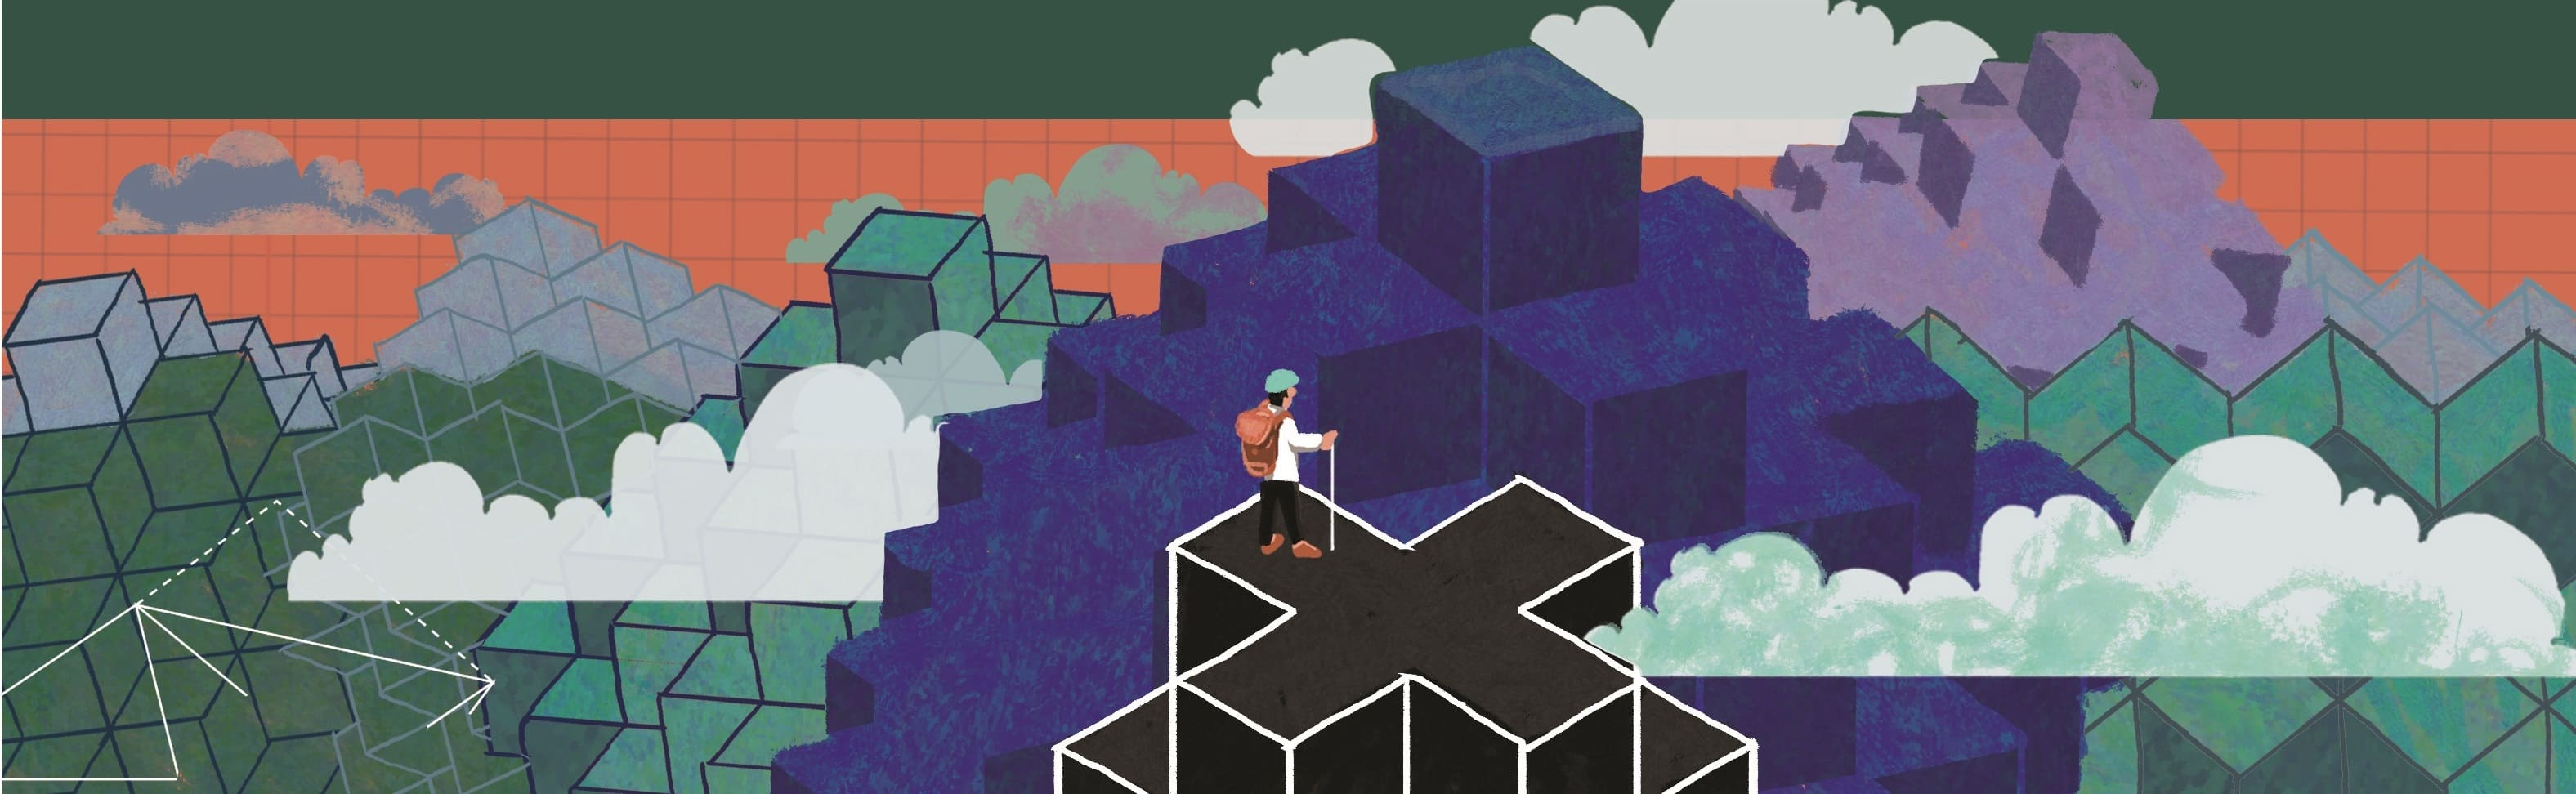
\includegraphics[width=19.3cm]{../thachthuctoanhoc/bannerthachthuc}}}
\centering
\vspace*{4cm}
\endgroup
\vspace*{-8pt}
\begin{tBox}
	\begin{itemize}[leftmargin = 13pt, itemsep = 1.0pt] 
		%		\item Mỗi bài toán đề xuất (kèm theo lời giải) cần được nêu rõ là bài sáng tác hay bài sưu tầm.
		\item Mỗi bài toán đề xuất (kèm theo lời giải) cần được nêu rõ là bài sáng tác hay bài sưu tầm (nếu là bài sưu tầm, cần ghi rõ nguồn).
		\item Bài giải cho mỗi bài toán cần được trình bày trong một file riêng hoặc
		một tờ giấy riêng.
		\item  Người đề xuất bài toán hoặc gửi bài giải cho các bài toán trong mục ``Thách thức kỳ này" cần ghi rõ họ, đệm, tên và nơi làm việc/học tập, số điện thoại liên hệ. Nếu là học sinh (hoặc sinh viên) cần ghi rõ là học sinh lớp mấy (hoặc sinh viên năm thứ mấy).
		\item Các bài toán trong mục Thách thức kỳ này hướng tới các độc giả là học sinh phổ thông; được phân chia thành các mức độ $B$, $A$, và được sắp xếp theo độ khó tăng dần, theo đánh giá chủ quan của Ban biên tập. Các bài toán mức độ $B$ không đòi hỏi các kiến thức vượt quá chương trình môn Toán cấp THCS; các bài toán mức độ $A$ không đòi hỏi các kiến thức vượt quá chương trình môn Toán cấp THPT.
		\item Cách thức gửi bài toán đề xuất hoặc lời giải: gửi file thu được bằng cách scan, ảnh chụp (rõ nét) của bản viết tay, hoặc được soạn thảo bằng các phần mềm Latex, Word tới \url{bbt@pi.edu.vn} hoặc gửi qua đường bưu điện tới Tòa soạn (xem địa chỉ tại bìa $2$).
		\item Hạn gửi lời giải cho các bài toán P$581$--P$590$: trước ngày $15/4/2022$.
	\end{itemize}
\end{tBox}
\begin{center}
	\vspace*{-5pt}
	\textbf{\color{thachthuctoanhoc}THÁCH THỨC KỲ NÀY}
	\vspace*{-5pt}
\end{center}
\begin{multicols}{2}
	\setlength{\abovedisplayskip}{4pt}
	\setlength{\belowdisplayskip}{4pt}
	{\color{thachthuctoanhoc}{\usefont{T5}{qag}{b}{n} P581.}}
	(Mức $B$) Xét năm số nguyên khác nhau $a,b,c,d,e$ sao cho tổng của ba số bất kì trong chúng lớn hơn tổng của hai số còn lại. Tìm giá trị nhỏ nhất của tổng 
	\begin{align*}
		S=abcd+abce+abde+acde+bcde.
	\end{align*}
	\begin{flushright}
		\textit{Nguyễn Đức Tấn, Tp. Hồ Chí Minh (st)}
	\end{flushright}
	{\color{thachthuctoanhoc}{\usefont{T5}{qag}{b}{n} P582.}}
	(Mức $B$) Bạn Tâm nghĩ trong đầu một số nguyên lớn hơn $2$ và nhỏ hơn $26$. Bạn An hỏi bạn Tâm ba câu hỏi sau, về số mà bạn Tâm nghĩ:  
	\vskip 0.05cm
	-- Số đó có phải là số chính phương không?
	\vskip 0.05cm
	-- Số đó có phải là số nguyên tố không?
	\vskip 0.05cm
	-- Số đó có chia hết cho $n$ không?, 
	\vskip 0.05cm
	trong đó, $n$ là một số tự nhiên chẵn có một chữ số, do An tự chọn. 
	\vskip 0.05cm
	Biết rằng, căn cứ câu trả lời của Tâm cho ba câu hỏi trên, An đã đoán ra được chính xác số Tâm nghĩ trong đầu. Hỏi, An đã chọn số $n$ nào, và số Tâm nghĩ là số nào?
	\begin{flushright}
		\textit{Đặng Hải Hà, Hưng Yên (st)}
	\end{flushright}
	{\color{thachthuctoanhoc}{\usefont{T5}{qag}{b}{n} P583.}}
	(Mức $B$) Giả sử $a,b$ là các số dương, sao cho $a+b+\dfrac1a+\dfrac1b$ và $a^3+b^3+\dfrac1{a^3}+\dfrac1{b^3}$ đều là các số hữu tỷ. Chứng minh rằng, $a^2+b^2+\dfrac1{a^2}+\dfrac1{b^2}$ cũng là một số hữu tỷ. 
	\begin{flushright}
		\textit{NguyễnTường Thanh, Nghệ An (st)}
	\end{flushright}
	{\color{thachthuctoanhoc}{\usefont{T5}{qag}{b}{n} P584.}}
	(Mức $B$) Cho tam giác $ABC$ cân tại $A$, có $I$ là tâm đường tròn nội tiếp. Các đường thẳng $BI$ và $AC$ cắt nhau tại $D$. Gọi $E$ là điểm đối xứng của $I$ qua $D$; $O$ là tâm đường tròn ngoại tiếp tam giác $BCE$. Chứng minh rằng $OD\perp AC$. 
		\begin{figure}[H]
		\centering
		\vspace*{-5pt}
		\captionsetup{labelformat= empty, justification=centering}
		\includegraphics[width=0.9\linewidth]{P584}
		\vspace*{-15pt}
	\end{figure}
	\begin{flushright}
		\textit{Nguyễn Trường Minh, Hải Dương (st)}
	\end{flushright}
	{\color{thachthuctoanhoc}{\usefont{T5}{qag}{b}{n} P585.}}
	(Mức $B$) Tìm tất cả các số tự nhiên $x,y,z$ thoả mãn $(y-z)^4+1=2^x yz$. 
	\begin{flushright}
		\textit{Hà Duy Hưng, Hà Nội}
	\end{flushright}
	{\color{thachthuctoanhoc}{\usefont{T5}{qag}{b}{n} P586.}}
	(Mức $B$) Cho $a,b,c$ là các số thực dương có tổng bằng $3$.  Chứng minh rằng 
	\begin{align*}
		2\left(\dfrac1a+\dfrac1b+\dfrac1c\right)\ge a^2+b^2+c^2+3.
	\end{align*}
	\begin{flushright}
		\textit{Nguyễn Đông Dương}
	\end{flushright}
	{\color{thachthuctoanhoc}{\usefont{T5}{qag}{b}{n} P587.}}
	(Mức $A$) Cho $a,b,c,d,e,f$ là $6$ số hạng liên tiếp trong dãy Fibonacci. Trong mặt phẳng toạ độ, lấy các điểm $A(a;b)$, $B(c;d)$, $C(e;f)$
	Tính diện tích của tam giác $ABC$.
	\vskip 0.05cm
	(Dãy Fibonacci $(F_n)$ được xác định như sau: $F_0=0$, $F_1=1$ và $F_{n+2}=F_{n+1}+F_n$ với mọi $n\ge0$).
	\begin{flushright}
		\textit{Phùng Hồ Hải, Hà Nội}
	\end{flushright}
	\columnbreak
	{\color{thachthuctoanhoc}{\usefont{T5}{qag}{b}{n} P588.}}
	(Mức $A$) Xét các số thực $x,y,z$, thoả mãn $(x-1)^2+(y+2)^2+(z-1)^2=300$. Tìm giá trị lớn nhất và nhỏ nhất của biểu thức 
	\begin{align*}
		P=[x^2]+[y^2]+[z^2].
	\end{align*}
	\begin{flushright}
		\textit{Vũ Hồng Phong, Bắc Ninh}
	\end{flushright}
	{\color{thachthuctoanhoc}{\usefont{T5}{qag}{b}{n} P589.}}
	(Mức $A$) Cho tam giác nhọn $ABC$ nội tiếp đường tròn $(O)$, có trực tâm $H$, và $M$ là trung điểm $BC$. Qua $H$, kẻ đường thẳng $d$ cắt các cạnh $AB,AC$ lần lượt tại $F,E$. Gọi $K$ là tâm đường tròn ngoại tiếp tam giác $AEF$ và $J$ là trung điểm $EF$. Các đường thẳng $AK,AJ$ theo thứ tự cắt $(O)$ tại các điểm thứ hai $L,G$. Chứng minh rằng $\widehat{MLG}=90^\circ$. 
	\begin{figure}[H]
		\centering
		\vspace*{-5pt}
		\captionsetup{labelformat= empty, justification=centering}
		\includegraphics[width=0.9\linewidth]{P589}
		\vspace*{-15pt}
	\end{figure}
	\begin{flushright}
		\textit{Đỗ Đại Phong, Tp. Huế}
	\end{flushright}
	{\color{thachthuctoanhoc}{\usefont{T5}{qag}{b}{n} P590.}}
	(Mức $A$) Cho biết, $\{1;2;3;4;5;6;7;8;9\}$ là tập hợp tất cả các hệ số của ba tam thức bậc hai $f(x),g(x),h(x)$. Hỏi, có thể xảy ra hay không, trường hợp ba tam thức đó có nghiệm hữu tỷ chung?
	\begin{flushright}
		\textit{Lê Phúc Lữ, Tp. Hồ Chí Minh}
	\end{flushright}
\end{multicols}

\newpage
\begin{center}
	{\large{\textbf{\color{thachthuctoanhoc}\color{thachthuctoanhoc}GIẢI BÀI KỲ TRƯỚC}}}
\end{center}
\begin{multicols}{2}
	\setlength{\abovedisplayskip}{4pt}
	\setlength{\belowdisplayskip}{4pt}
	{\color{thachthuctoanhoc}{\usefont{T5}{qag}{b}{n} P551.}}
	(Mức $B$) Tìm số có năm chữ số  $\overline{abcde}$, thỏa mãn:
	\begin{align*}
		\overline {ab,c} :\overline {bde}  = 0,9.
	\end{align*}
	\textbf{\color{thachthuctoanhoc}Lời giải} (\textit{dựa theo đa số lời giải Tòa soạn nhận được từ bạn đọc})\textbf{\color{thachthuctoanhoc}.}
	\vskip 0.05cm
	Từ giả thiết, ta có:
	\begin{align*}
		\overline{abc} = 9 \cdot \overline{bde}. \tag{$1$}
	\end{align*}
	Từ đó, do $\overline{abc} \le 999$,  suy ra $\overline{bde} \le 111$. Do đó, $b = 1$. Vì thế, theo ($1$), ta có:
	\begin{align*}
		\overline{a1c} = 9 \cdot \overline{1de};\tag{$2$}
	\end{align*}
	suy ra, $\overline{a1c} \ge 9 \cdot 100 = 900$  (do $\overline{1de \ge 100}$). Do đó, $a = 9$. Vì thế, theo ($2$), ta có:
	\begin{align*}
		\overline{91c} = 9\cdot \overline{1de};
	\end{align*}
	suy ra, $\overline{91c}$ chia hết cho $9$. Do đó, ($9 + 1 + c$) chia hết cho $9$; suy ra, $1 + c$ chia hết cho $9$. Mà $0 \le c \le 9$, nên $c = 8$. Suy ra
	\begin{align*}
		\overline {1de}  = \overline {91c} :9 = 918:9 = 102.
	\end{align*}
	Vì vậy, $d = 0$ và $e = 2$. Do đó, số phải tìm là $91802$.
	\vskip 0.05cm
	\textbf{\color{thachthuctoanhoc}Bình luận và Nhận xét}
	\vskip 0.05cm
	$\pmb{1.}$ Trong số các lời giải Tạp chí nhận được từ bạn đọc, rất tiếc, có một lời giải sai, do người giải bài quan niệm rằng, có thể xảy ra trường hợp $b = 0$.
	\vskip 0.05cm
	(\textbf{\color{thachthuctoanhoc}Lưu ý:} $\overline{xyz}$  ký hiệu số có ba chữ số; một cách khái quát,  $\overline {{x_1}{x_2} \ldots {x_n}} $, $n \in \mathbb{N^*}$, ký hiệu số có $n$ chữ số.)
	\vskip 0.05cm
	$\pmb{2.}$ Bên cạnh lời giải sai nêu trên, có một lời giải không được coi là lời giải hoàn chỉnh, do người giải bài chỉ nêu hướng giải bài toán (thử lần lượt $12$ trường hợp có thể xảy ra với $\overline{bde}$: $\overline{bde}= 100$, $\overline{bde} = 101$,    $\ldots$, $\overline{bde}= 111$), mà không nêu cách thực hiện hướng giải đó (thử như thế nào?).
	\begin{flushright}
		\textbf{\color{thachthuctoanhoc}Lưu Thị Thanh Hà}
	\end{flushright}
	{\color{thachthuctoanhoc}{\usefont{T5}{qag}{b}{n} P552.}}
	(Mức $B$) Xác định số nguyên lớn nhất không vượt quá số
	\begin{align*}
		A = \frac{{{{2020}^{2021}} + {{2021}^{2022}}}}{{{{2020}^{2020}} + {{2021}^{2021}}}}.
	\end{align*}
	\textbf{\color{thachthuctoanhoc}Lời giải} (\textit{của bạn Nguyễn Đức Sơn, lớp $10$\linebreak Toán, trường THPT chuyên Nguyễn Tất Thành, tỉnh Kon Tum})\textbf{\color{thachthuctoanhoc}.}
	\vskip 0.05cm
	Đặt $a = {2020^{2020}}$, $b = {2021^{2021}}$;  ta có: $a, b > 0$ và
	\begin{align*}
		A = \frac{{2020a + 2021b}}{{a + b}} = 2020 + \frac{b}{{a + b}}.
	\end{align*}
	Suy ra, $2020 < A < 2021$ (do  $0 < \frac{b}{{a + b}} < 1$). Vì thế, số nguyên lớn nhất không vượt quá $A$ là $2020$.
	\vskip 0.05cm
	\textbf{\color{thachthuctoanhoc}Bình luận và Nhận xét}
	\vskip 0.05cm
	$\pmb{1.}$ Số nguyên lớn nhất không vượt quá số thực $x$ được gọi là \textit{phần nguyên} của $x$. Sử dụng khái niệm này, ta có thể phát biểu đề bài một cách ngắn gọn, như sau: “Tìm phần nguyên của số 
	\begin{align*}
		A = \frac{{{{2020}^{2021}} + {{2021}^{2022}}}}{{{{2020}^{2020}} + {{2021}^{2021}}}}. \text{\color{black}"}
	\end{align*}
	$\pmb{2.}$ Dễ thấy, trong Lời giải trên, thay $2020$ bởi $n$, với $n$ là một số nguyên dương tùy ý, ta sẽ có một chứng minh ngắn gọn cho kết quả tổng quát sau:
	\vskip 0.05cm
	“\textit{Với mọi số nguyên dương $n$, phần nguyên của số 
	\begin{align*}
		\frac{{{n^{n + 1}} + {{\left( {n + 1} \right)}^{n + 2}}}}{{{n^n} + {{\left( {n + 1} \right)}^{n + 1}}}}
	\end{align*}  
	bằng $n$.}”
	\vskip 0.05cm
	$\pmb{3.}$ Trong số các lời giải Tạp chí nhận được từ bạn đọc, rất tiếc, có hai lời giải sai, do người giải bài đã mắc lỗi kiến thức cơ bản. Cụ thể, các bạn đó đã lập luận rằng, với $a$ là số nguyên và $x$ là số thực, từ $x < a$ suy ra phần nguyên của $x$ bằng $a - 1$. Có thể thấy, lập luận đó là một lập luận sai qua, chẳng hạn, ví dụ đơn giản sau: $1,1 < 3$, nhưng $2 (= 3 - 1)$ không phải là phần nguyên của $1,1$ (tức, không phải là số nguyên lớn nhất không vượt quá $1,1$).
	\vskip 0.05cm
	(\textbf{\color{thachthuctoanhoc}Lưu ý:} \textit{Số nguyên $a$ là phần nguyên của số thực $x$ \textbf{\color{thachthuctoanhoc}khi và chỉ khi} $a \le x < a + 1$.})
	\begin{flushright}
		\textbf{\color{thachthuctoanhoc}Lưu Thị Thanh Hà}
	\end{flushright}
	{\color{thachthuctoanhoc}{\usefont{T5}{qag}{b}{n} P553.}}
	(Mức $B$) Một bức tường hình vuông được ốp khít bởi các viên gạch hình chữ nhật kích thước $7$cm $\times$ $13$cm (các viên gạch không bị cắt ra, không bị sứt mẻ khi ốp), sao cho tất cả các cạnh có độ dài $7$cm song song với chiều ngang của bức tường, và tất cả các cạnh có độ dài $13$cm song song với chiều cao của bức tường.
	\vskip 0.05cm
	Biết rằng, chiều cao của bức tường lớn hơn $2$m và nhỏ hơn $3$m; giá mỗi viên gạch là $15{.}000$ đồng. Hỏi số tiền gạch phải bỏ ra là bao nhiêu? (Bỏ qua diện tích của vật liệu khác, khi ốp gạch.)
	\vskip 0.05cm
	\textbf{\color{thachthuctoanhoc}Lời giải} (\textit{dựa theo lời giải của các bạn: Nguyễn Hùng Cường, lớp $8$A$4$, trường THCS Nhơn Mỹ, Thị xã An Nhơn, tỉnh Bình Định, và Đặng Quang Phúc, lớp $10$ Toán $1$, trường THPT chuyên Lương Văn Chánh, tỉnh Phú Yên}).
	\vskip 0.05cm
	Đổi đơn vị: $2$m $=$ $200$cm, $3$m $=$ $300$cm.
	\vskip 0.05cm
	Từ các giả thiết về việc ốp bức tường bằng các viên gạch, suy ra:
	\vskip 0.05cm
	-- Các viên gạch ốp trên tường được chia \linebreak thành các hàng dọc, chạy song song với, hoặc dọc theo, chiều cao của bức tường, và số viên gạch ở mỗi hàng là như nhau;
	\vskip 0.05cm
	-- Độ dài chiều cao của bức tường (tính theo đơn vị cm) gấp $13$ lần số viên gạch của một hàng, và độ dài chiều ngang của bức tường (tính theo đơn vị cm) gấp $7$ lần số hàng gạch.
	\vskip 0.05cm
	Do đó, gọi $m$ là số hàng gạch (được nói ở trên) và $n$ là số viên gạch của một hàng, $m,m \in \mathbb{N^*}$,  ta có $13n$ (cm) và $7m$ (cm), tương ứng, là độ dài chiều cao và độ dài chiều ngang của bức tường. Từ đây, do bức tường là hình vuông và độ dài chiều cao của nó lớn hơn $200$cm, nhỏ hơn $300$cm, ta có:
	\begin{align*}
	\hspace*{20pt}\begin{cases}
			7m = 13n \hspace*{112pt} \text{\color{black}($\color{thachthuctoanhoc}1$)}\\
			200 < 13n < 300. \hspace*{73pt} \text{\color{black}($\color{thachthuctoanhoc}2$)}
		\end{cases}
	\end{align*}
	Từ ($1$), do $(13, 7) = 1$, suy ra $n \,\,\vdots\,\, 7$. \hfill ($3$)
	\vskip 0.05cm
	Từ ($2$), với lưu ý $n \in \mathbb{N^*}$,  suy ra  
	\begin{align*}
		16 \le n \le 23. \tag{$4$}
	\end{align*}
	Từ ($3$) và ($4$), ta được $n = 21$. Do đó, theo ($1$), ta có:
	\begin{align*}
		m = \frac{{13 \cdot 21}}{7} = 39.
	\end{align*}
	Suy ra, số viên gạch được dùng ốp tường là:
	\begin{align*}
		21 \cdot 39 = 819 \,\,\text{\color{black} (viên).}
	\end{align*}
	Vì thế, số tiền phải bỏ ra để mua gạch ốp tường là:
	\begin{align*}
		15{.}000 \cdot 819 = 12{.}285{.}000 \,\,\text{\color{black} (đồng).}
	\end{align*}
	\textbf{\color{thachthuctoanhoc}Bình luận và Nhận xét}
	\vskip 0.05cm
	Tất cả các lời giải Tạp chí nhận được từ bạn đọc đều là lời giải đúng.
	\begin{flushright}
		\textbf{\color{thachthuctoanhoc}Lê Huy}
	\end{flushright}
	{\color{thachthuctoanhoc}{\usefont{T5}{qag}{b}{n} P554.}}
	(Mức $B$) Cho $x, y, z$ là các số thực dương, thỏa mãn ${x^2} + {y^2} + {z^2} = 1$.  Chứng minh rằng
	\begin{align*}
		\frac{1}{{1 + yz}} \le \frac{{\sqrt 2 }}{{x + y + z}}.
	\end{align*}
	\textbf{\color{thachthuctoanhoc}Lời giải.}
	\vskip 0.05cm
	$\bullet$ \textbf{\color{thachthuctoanhoc}Cách} $\pmb{1}$ (\textit{dựa theo lời giải của các bạn: Nguyễn Đức Sơn, lớp $10$ Toán, trường THPT chuyên Nguyễn Tất Thành, tỉnh Kon Tum, và Trần Văn Quân, lớp $12$ Toán $1$, trường THPT chuyên Hưng Yên, tỉnh Hưng Yên})\textbf{\color{thachthuctoanhoc}.}
	\vskip 0.05cm
	Ký hiệu ($1$) là bất đẳng thức cần chứng minh của đề bài.
	\vskip 0.05cm
	Do $x, y, z > 0$ nên ta có:
	\begin{align*}
		&(1) \\
		\Leftrightarrow \,&\sqrt 2 \left( {1 + yz} \right) \ge x + y + z\\
		\Leftrightarrow \,&2{\left( {1 + yz} \right)^2} \ge {\left( {x + y + z} \right)^2}\\
		\Leftrightarrow \,&2\left( {{x^2} + {y^2} + {z^2} + 2yz + {y^2}{z^2}} \right)\\
		&\ge {x^2} + {y^2} + {z^2} + 2\left( {xy + yz + zx} \right) \\
		& (\text{\color{black}do } {x^2} + {y^2} + {z^2} = 1)\\
		\Leftrightarrow \,&{x^2} \!+\! {y^2} \!+\! {z^2}\! -\! 2xy \!+\! 2yz \!-\! 2zx \!+\! 2{y^2}{z^2} \ge 0\\
		\Leftrightarrow \,&{\left( {x - y - z} \right)^2} + 2{y^2}{z^2} \ge 0. \tag{$2$}
	\end{align*}
	($2$) là bất đẳng thức đúng. Vì thế, bất đẳng thức ($1$) được chứng minh.
	\vskip 0.05cm
	Do $y, z > 0$ nên dấu đẳng thức ở ($2$) không thể xảy ra. Vì thế, \textit{dấu đẳng thức ở \textrm{($1$)} cũng không thể xảy ra}.
	\vskip 0.05cm
	$\bullet$ \textbf{\color{thachthuctoanhoc}Cách} $\pmb{2}$ (\textit{dựa theo cách giải của các bạn Nguyễn Hải Đăng và Nguyễn Trường Duy, lớp $11$T$1$, THPT chuyên Nguyễn Quang Diêu, tỉnh Đồng Tháp})\textbf{\color{thachthuctoanhoc}.}
	\vskip 0.05cm
	Ta có:
	\begin{align*}
			&\left( {x + y + z} \right)^2 \\
			= \,&1 \!+\! 2x\left( {y \!+\! z} \right) \!+\! 2yz\,\,\left(\text{\color{black}do \,}{x^2} + {y^2} + {z^2} = 1 \right)\\
			 \le\,& 1 + {x^2} + {\left( {y + z} \right)^2} + 2yz\\
			 &\left({{\text{\color{black}do \,}}{{\left( {x - \left( {y + z} \right)} \right)}^2} \ge 0\quad\forall x,y,z \in \mathbb{R}} \right)\\
			 = \,&2 + 4yz\quad\left( {\text{\color{black}do \,}{x^2} + {y^2} + {z^2} = 1} \right)\\
			 < \,&2 + 4yz + 2{y^2}{z^2}\quad\left( {\text{\color{black}do \,}y,z \ne 0} \right)\\
			 = \,&2{\left( {1 + yz} \right)^2}.
	\end{align*}
	Từ đó, do $x, y, z > 0$, suy ra
	\begin{align*}
		x + y + z < \sqrt 2 \left( {1 + yz} \right);
	\end{align*}
	do đó
	\begin{align*}
		\frac{1}{{1 + yz}} < \frac{{\sqrt 2 }}{{x + y + z}}.
	\end{align*}
	Ta có điều phải chứng minh theo yêu cầu đề bài.
	\vskip 0.05cm
	Chứng minh trên đây cho thấy \textit{dấu đẳng thức ở bất đẳng thức của đề bài không thể xảy ra.}
	\vskip 0.05cm
	\textbf{\color{thachthuctoanhoc}Bình luận và Nhận xét}
	\vskip 0.05cm
	$\pmb{1.}$ Ngoài hai cách chứng minh nêu trên, nhờ việc sử dụng các bất đẳng thức cơ bản (như: bất đẳng thức Cauchy (Cô--si), bất đẳng thức Cauchy -- Buniacovski), ta còn có các cách chứng minh ngắn gọn khác cho bất đẳng thức của đề bài.
	\vskip 0.05cm
	$\pmb{2.}$ Hai lời giải trên đây cho thấy, bất đẳng thức của đề bài vẫn đúng, nếu thay ràng buộc “$x, y, z > 0$” bởi ràng buộc “$x + y + z > 0$ và $yz > -1$”. Ràng buộc mới vừa nêu chẳng những cho thấy một mở rộng vùng đúng của bất đẳng thức ở đề bài, mà còn làm cho bất đẳng thức đó trở thành một bất đẳng thức chặt (do khi đó, dấu đẳng thức có thể xảy ra).
	\vskip 0.05cm
	$\pmb{3.}$ Trong số các bạn đọc đã gửi lời giải tới Tạp chí, không ít bạn đã khẳng định dấu đẳng thức ở bất đẳng thức của đề bài có thể xảy ra!? Tuy nhiên, do đề bài không yêu cầu kiểm tra khả năng xảy ra đẳng thức, nên tất cả các lời giải có phần chứng minh đúng bất đẳng thức của đề bài vẫn được coi là lời giải đúng và hoàn chỉnh.
	\vskip 0.05cm
	$\pmb{4.}$ Trong số các lời giải Tạp chí đã nhận được từ bạn đọc, có hai lời giải sai, do người giải bài đã sử dụng các biến đổi, đánh giá sai dưới đây:
	\vskip 0.05cm
	$\bullet$ ${x^2} + {y^2} + {z^2} = {\left( {x + y + z} \right)^2}$;
	\vskip 0.05cm
	$\bullet$ ${x^2} + {y^2} + {z^2} \ge {x^2} + {\left( {y + z} \right)^2}$.
	\begin{flushright}
		\textbf{\color{thachthuctoanhoc}Lê Huy}
	\end{flushright}
	{\color{thachthuctoanhoc}{\usefont{T5}{qag}{b}{n} P555.}}
	(Mức $B$) Cho tam giác $ABC$, với $CB < CA$, nội tiếp đường tròn $(O)$, và ngoại tiếp đường tròn $(I)$. $E$ là điểm chính giữa của cung $BC$ không chứa $A$ của đường tròn $(O)$. Đường tròn đi qua hai điểm $A$, $I$, và tiếp xúc với $AC$, cắt $(O)$ tại điểm thứ hai $F$ (khác $A$). Gọi $K$ là giao điểm của $EF$ và $BC$; $H$ là giao điểm của $AB$ và $IK$. Chứng minh rằng, $FH$ là phân giác của góc $IFK$.
	\vskip 0.05cm
	\textbf{\color{thachthuctoanhoc}Lời giải} (\textit{của người chấm bài})\textbf{\color{thachthuctoanhoc}.}
		\begin{figure}[H]
		\vspace*{-5pt}
		\centering
		\captionsetup{labelformat= empty, justification=centering}
		\includegraphics[width=1\linewidth]{P555}
		\vspace*{-10pt}
	\end{figure}
	Gọi $D$ là giao điểm của đoạn thẳng $AE$ và đoạn thẳng $BC$. Do $E$ là điểm chính giữa của cung $BC$ không chứa $A$ của đường tròn $(O)$ nên $AE$ là phân giác trong của $\angle BAC$.  Vì thế, bốn điểm $A, I, D, E$ thẳng hàng.
	\vskip 0.05cm
	Giả sử $K$ thuộc tia đối của tia $BC$. Trường hợp $K$ thuộc tia đối của tia $CB$ được xét tương tự.
	\vskip 0.05cm
	Do đường tròn $(AIF)$ tiếp xúc với $AC$ nên
	\begin{align*}
		\angle IFA = \angle IAC = \angle EBC. \tag{$1$}
	\end{align*}
	Do đó, xét tam giác $AFI$ và đường tròn $(O)$, ta có:
	\begin{align*}
		\angle FID &= \angle IAF + \angle IFA \\
		&= \angle FBE + \angle EBC = \angle FBC.
	\end{align*}
	Suy ra, $FBID$ là tứ giác nội tiếp.  \hfill ($2$)
	\vskip 0.05cm
	Xét tam giác $BFK$ và đường tròn $(O)$, ta có:
	\begin{align*}
		\angle FKD &= \angle FBC - \angle BFK \\
		&= \angle FAC - \angle BAE \\
		&= \angle FAC - \angle CAE = \angle FAD.
	\end{align*}
	Suy ra, $FKAD$ là tứ giác nội tiếp. \hfill ($3$)
	\vskip 0.05cm
	Tiếp theo, ta có:
	\begin{align*}
			\angle AKB &= \angle AKF - \angle FKD \\
			&= \angle FDE - \angle FAD\,\,\,\left(\text{\color{black}do ($\color{thachthuctoanhoc}3$)} \right)\\
			 &= \angle AFD = \angle AFI + \angle IFD\\
			 &= \angle IAC + \angle IBC\,\,\left(\text{\color{black}do ($\color{thachthuctoanhoc}1$) và ($\color{thachthuctoanhoc}2$)} \right)\\
			 &= \angle IAB + \angle IBA\,\,\,(\text{\color{black} do $\color{thachthuctoanhoc}I$ là tâm đường}\\
			  &\quad\,\text{\color{black}tròn nội tiếp tam giác}\,\, ABC)\\
			 &= \angle BID.
	\end{align*}
	Suy ra, $AIBK$ là tứ giác nội tiếp.                                                                                                            \hfill ($4$)
	\vskip 0.05cm
	Gọi $P$ là giao điểm thứ hai, khác $C$, của $IC$ và $(O)$; ta có $P$ là tâm đường tròn ngoại tiếp tam giác $AIB$. Do đó, theo ($4$), $P$ là tâm đường tròn ngoại tiếp tứ giác $AIBK$. Suy ra,\linebreak $PI = PK$. \hfill                                  ($5$)
	\vskip 0.05cm
	Hơn nữa, với lưu ý tới ($3$) và ($4$), ta có:
	\begin{align*}
		\angle FPC &= \angle FAC = \angle FAE + \angle EAC \\
		&= \angle FKD + \angle EAB \\
		&= \angle FKD + \angle IKB = \angle FKI.
	\end{align*}
	Do đó, $FKPI$ là tứ giác nội tiếp. Từ đây và ($5$) suy ra, $FP$ là phân giác của $\angle IFK$                              \hfill ($6$)
	\vskip 0.05cm
	Mặt khác, do $AB$ là trục đẳng phương của đường tròn $(AIBK)$ và đường tròn $(O)$, $IK$ là trục đẳng phương của đường tròn $(AIBK)$ và đường tròn $(FKPI)$, nên $H$ là tâm đẳng phương của ba đường tròn $(AIBK)$, $(FKPI)$ và $(O)$. Vì thế, trục đẳng phương $FP$ của $(FKPI)$ và $(O)$ đi qua $H$. Do đó, theo $(6)$, $FH$ là phân giác của $\angle IFK$.
	\vskip 0.05cm
	Ta có điều phải chứng minh theo yêu cầu đề bài.
	\vskip 0.05cm
	\textbf{\color{thachthuctoanhoc}Bình luận và Nhận xét}
	\vskip 0.05cm
	$\pmb{1.}$ Bằng cách tương tự Lời giải trên, bạn đọc có thể giải được bài toán khái quát sau của bài đã ra:
	\vskip 0.05cm
	\textbf{\color{thachthuctoanhoc}Bài toán khái quát.} \textit{Cho tam giác $ABC$ nội tiếp đường tròn $(O)$, và ngoại tiếp đường tròn $(I)$. $E$ là điểm chính giữa của cung $BC$ không chứa $A$ của đường tròn $(O)$. Trên cạnh $AC$, lấy một điểm $P$ tùy ý. Đường tròn ngoại tiếp tam giác $AIP$ cắt $(O)$ tại điểm thứ hai $F$ (khác $A$). Gọi $K$ là giao điểm của $EF$ và $BC$; $H$ là giao điểm của $AB$ và $IK$. Gọi $\alpha$ là số đo của góc tạo bởi $FH$ và phân giác trong của góc $IFK$. Chứng minh rằng, $\angle AIP = 2\alpha$.}
	\vskip 0.05cm
	$\pmb{2.}$ Tất cả các lời giải Tạp chí nhận được từ bạn đọc đều là lời giải đúng.
	\begin{flushright}
		\textbf{\color{thachthuctoanhoc}Trần Quang Hùng}
	\end{flushright}
	{\color{thachthuctoanhoc}{\usefont{T5}{qag}{b}{n} P556.}}
	(Mức $B$) Cho bảng ô vuông kích thước $4 \times 4$. Điền $16$ số $1, 2, 2^2, \ldots,2^{15}$ vào các ô vuông con của bảng, sao cho ở mỗi ô được điền đúng một số, và mỗi số được điền vào đúng một ô. Cho phép thay đổi các số có trong bảng, theo quy tắc: Mỗi lần, chọn tùy ý một bảng con $2 \times 2$ của bảng đã cho, rồi cộng thêm vào mỗi số có trong bảng con đó cùng một số thực tùy ý.
	\vskip 0.05cm
	Chứng minh rằng, bằng cách thực hiện một số hữu hạn lần liên tiếp phép thay đổi số nói trên đối với bảng số ban đầu, ta không thể thu được bảng $4 \times 4$, mà tất cả các số trong bảng đều bằng nhau.
	\vskip 0.05cm
	\textbf{\color{thachthuctoanhoc}Lời giải} (\textit{dựa theo cách giải của bạn Trần Văn Quân, lớp $12$ Toán $1$, trường THPT chuyên Hưng Yên, tỉnh Hưng Yên})\textbf{\color{thachthuctoanhoc}.}
	\vskip 0.05cm
	Gọi $S$ là tổng tất cả các số được điền vào các ô vuông con của bảng.
	\vskip 0.05cm
	Tô màu các ô vuông con của bảng đã cho, bởi hai màu xanh, trắng, như ở hình dưới đây.
			\begin{figure}[H]
		\vspace*{-5pt}
		\centering
		\captionsetup{labelformat= empty, justification=centering}
		\includegraphics[width=0.55\linewidth]{P556}
		\vspace*{-10pt}
	\end{figure}
	Xét một cách điền số tùy ý, thỏa mãn điều kiện đề bài.
	\vskip 0.05cm
	Ký hiệu $X_0$  và $T_0$  tương ứng là tổng các số được điền vào ô xanh và tổng các số được điền vào ô trắng.
	\vskip 0.05cm
	Với mỗi số nguyên dương $k$, ký hiệu $X_k$  và $T_k$  tương ứng là tổng các số nằm ở ô xanh và tổng các số nằm ở ô trắng, sau lần thực hiện phép thay đổi số thứ $k$.
	\vskip 0.05cm
	Dễ thấy, mỗi bảng con $2 \times 2$ của bảng đã cho đều có đúng hai ô xanh và hai ô trắng. Do đó, sau mỗi lần thực hiện phép thay đổi số, tổng các số nằm ở ô xanh và tổng các số nằm ở ô trắng, của bảng đã cho, đều được tăng lên một lượng như nhau. Vì thế, ta có:
	\begin{align*}
		X_k - T_k = X_0 - T_0, \tag{$*$}
	\end{align*}
	với mọi $k \in \mathbb{N^*}$.
	\vskip 0.05cm
	Giả sử tồn tại một cách điền số, thỏa mãn điều kiện đề bài, sao cho nhờ việc thực hiện một số hữu hạn lần liên tiếp phép thay đổi số đối với bảng số ban đầu, ta có thể thu được bảng $4 \times 4$, mà tất cả các số trong bảng đều bằng nhau. Theo $(*)$, với cách điền số này, ta có:
	\begin{align*}
		{X_0} - {T_0} = 0.
	\end{align*}
	Suy ra
	\begin{align*}
		S = {X_0} + {T_0} = 2{X_0},
	\end{align*}
	là điều vô lý, do $X_0$  là một số nguyên và
	\begin{align*}
		S = 1 + 2 + {2^2} +  \cdots  + {2^{15}}
	\end{align*}
	là một số lẻ.
	\vskip 0.05cm
	Điều vô lý nhận được cho thấy, điều giả sử nêu trên là sai. Vì thế, ta có điều phải chứng minh theo yêu cầu đề bài.
	\vskip 0.05cm
	\textbf{\color{thachthuctoanhoc}Bình luận và Nhận xét}
	\vskip 0.05cm
	$\pmb{1.}$ Trong lời giải của mình, bạn \textit{Trần Văn Quân} đã khai thác đẳng thức $X_0 - T_0 = 0$,  hay $X_0 = T_0$,  theo một cách nhìn khác, ít “bình dân” hơn (và vì thế, ít gần gũi hơn đối với đại đa số học sinh cấp THCS) so với cách khai thác được thể hiện ở Lời giải trên đây. Cụ thể, bạn Quân đã nhìn nhận rằng, đẳng thức đó cho thấy, tập hợp tất cả các số, được dùng để điền vào bảng, có thể được phân chia thành hai tập con khác rỗng, sao cho tổng tất cả các số thuộc tập con này bằng tổng tất cả các số thuộc tập con kia. Từ cách nhìn này và nhận xét
	\begin{align*}
		1 + 2 + {2^2} +  \cdots  + {2^{14}} = {2^{15}} - 1 < {2^{15}},
	\end{align*}
	hiển nhiên dễ dàng tìm ra điều vô lý, khi giả sử điều ngược lại với kết luận của bài ra.
	\vskip 0.05cm
	$\pmb{2.}$ Cách nhìn nêu trên của bạn Quân cho ta thấy, kết luận của bài ra không phải là một \linebreak tính chất “độc quyền” của nhóm $16$ số nguyên dương đã nêu trong đề bài. Cụ thể, \textit{kết luận của bài ra vẫn đúng, chí ít, khi $16$ số được dùng để điền vào các ô vuông con của bảng $4 \times 4$ là $16$ số thực \textbf{\color{thachthuctoanhoc}không} đồng thời bằng nhau tất cả, và thỏa mãn điều kiện: số lớn nhất trong $16$ số lớn hơn tổng của $15$ số còn lại.}
	\vskip 0.05cm
	$\pmb{3.}$ Lời giải của bạn Trần Văn Quân là lời giải duy nhất, mà Tạp chí đã nhận được từ bạn đọc, cho tới thời điểm bản thảo vào nhà in.
	\begin{flushright}
		\textbf{\color{thachthuctoanhoc}Nguyễn Khắc Minh}
	\end{flushright}
	{\color{thachthuctoanhoc}{\usefont{T5}{qag}{b}{n} P557.}}
	(Mức $A$) Cho $a, b, c$ là các số thực dương tùy ý, và cho $x, y, z$ là các số thực dương có tổng bằng $1$. Đặt $M = \max\{a, b, c\}$ và $m = \min\{x, y, z\}$. Chứng minh rằng
		\begin{align*}
		&M-(xa+y b+z c) \\
		\ge&\dfrac m2\!\!\left(\!\!(\!\sqrt{a}\!-\!\!\sqrt{b})^{2}\!\!+\!(\sqrt{b}\!-\!\!\sqrt{\!c})^{2}\!+\!\!(\sqrt{\!c}\!-\!\sqrt{a})^{2}\!\right).
	\end{align*}

	\columnbreak
	\textbf{\color{thachthuctoanhoc}Lời giải} (\textit{của người chấm bài})\textbf{\color{thachthuctoanhoc}.}
	\vskip 0.05cm
	Dễ thấy, không mất tính tổng quát, có thể giả sử $a \ge b \ge c > 0$.\hfill                                                              ($1$)
	\vskip 0.05cm
	Khi đó, ta có:
	\begin{align*}
		M \!=\! a \!=\! a\left( {x \!+\! y \!+\! z} \right)\,\,\left( {{\text{\color{black}do\, }}x + y + z = 1} \right).
	\end{align*}
	Do đó
	\begin{align*}
		M - \left( {xa + yb + zc} \right) = y\left( {a - b} \right) + z\left( {a - c} \right).
	\end{align*}
	Vì thế, bất đẳng thức cần chứng minh, theo yêu cầu đề bài, trở thành:
	\begin{align*}
		&y\left( {a - b} \right) + z\left( {a - c} \right) \\
		\ge& \frac{m}{2}\!\!\left(\!(\!\sqrt a  \!-\!\! \sqrt b)^2 \!\!+\! (\!\sqrt b  \!-\! \sqrt c )^2 \!+\! (\!\sqrt c  \!-\! \sqrt a)^2\!\! \right)\!,
	\end{align*}
	hay
	\begin{align*}
		&y\left( {a - b} \right) + z\left( {a - c} \right) \\
		\ge \,&m\!\!\left(\!\!(a \!+\! b \!+\! c \!) \!-\! (\!\!\sqrt {ab}  \!+\! \sqrt {bc}  \!+\! \sqrt {ca})\!\! \right)\!\!. \tag{$2$}
	\end{align*}
	Do $m = \min\{x, y, z\}$ nên
	\begin{align*}
		y\left( {a \!-\! b} \right)\! +\! z\left( {a \!-\! c} \right) &\ge m\left( {a \!-\! b} \right) \!+\! m\left( {a \!-\! c} \right) \\
		&= m\left( {2a - b - c} \right). \tag{$3$}
	\end{align*}
	Tiếp theo, do ($1$) nên
	\begin{align*}
		\sqrt {ab}  + \sqrt {bc}  + \sqrt {ca} & \ge \sqrt {{b^2}}  + \sqrt {{c^2}}  + \sqrt {{c^2}}  \\
		&= b \!+\! 2c = 2b \!+\! 2c \!-\! b \\
		&\ge 2b + 2c - a.
	\end{align*}
	Từ đó, do $m > 0$, suy ra
	\begin{align*}
		&m\left( {\left( {a + b + c} \right) - \left( {\sqrt {ab}  + \sqrt {bc}  + \sqrt {ca} } \right)} \right) \\
		\le \,&m\left( {\left( {a + b + c} \right) - \left( {2b + 2c - a} \right)} \right) \\
		=\,& m\left( {2a - b - c} \right). \tag{$4$}
	\end{align*}
	Từ ($3$) và ($4$), hiển nhiên, thu được ($2$). Vì vậy, ta có điều phải chứng minh theo yêu cầu đề bài.
	\vskip 0.05cm
	\textbf{\color{thachthuctoanhoc}Bình luận và Nhận xét}
	\vskip 0.05cm
	$\pmb{1.}$ Sử dụng ý tưởng của Lời giải trên, bạn đọc có thể chứng minh được bất đẳng thức chặt hơn bất đẳng thức của đề bài, dưới đây:
	\begin{align*}
		&M - (ax + by + cz)\\
		 \ge\,& \frac{{m\left( {{{(a - b)}^2} + {{(b - c)}^2} + {{(c - a)}^2}} \right)}}{{a + b + c}} \\
		\ge\,& \frac{m}{2}\!\!\left(\!\!(\!\sqrt a  \!-\! \sqrt b)^2 \!\!+\!\! (\!\sqrt b  \!-\!\! \sqrt c)^2 \!\!+\!\! (\!\sqrt c  \!-\! \sqrt a)^2\!\!\right)\!\!.
	\end{align*}
	$\pmb{2.}$ Tạp chí đã nhận được ba lời giải từ bạn đọc; cả ba lời giải này đều là lời giải đúng.
	\begin{flushright}
		\textbf{\color{thachthuctoanhoc}Võ Quốc Bá Cẩn}
	\end{flushright}
	{\color{thachthuctoanhoc}{\usefont{T5}{qag}{b}{n} P558.}}
	(Mức $A$) Cho tam giác $ABC$ nội tiếp đường tròn $(O)$, và không cân tại $A$. Gọi $H$ là trực tâm của tam giác đó, và gọi $M$ là trung điểm cạnh $BC$. Đường thẳng đi qua $A$, và vuông góc với $AM$, cắt lại đường tròn $(O)$ tại điểm $D$ (khác $A$), và cắt lại đường tròn đường kính $AH$ tại điểm $E$ (khác $A$). Chứng minh rằng, $A$ là trung điểm của $DE$.
	\vskip
	 0.05cm
	\textbf{\color{thachthuctoanhoc}Lời giải} (\textit{của người chấm bài})\textbf{\color{thachthuctoanhoc}.}
	\vskip 0.05cm
	Trước hết, nhắc lại kết quả cơ bản sau:
	\vskip 0.05cm
	\textbf{\color{thachthuctoanhoc}Bổ đề.} Cho tam giác $XYZ$ với trực tâm $T$, nội tiếp đường tròn $(O)$. Gọi $U$ là điểm đối xứng với $T$ qua trung điểm của $YZ$, ta có $XU$ là một đường kính của $(O)$.
	\vskip 0.05cm
	\textit{Trở lại bài toán.}
		\begin{figure}[H]
		\vspace*{-5pt}
		\centering
		\captionsetup{labelformat= empty, justification=centering}
		\includegraphics[width=0.9\linewidth]{P558}
		\vspace*{-10pt}
	\end{figure}
	Gọi $A'$  là điểm đối xứng với $H$ qua $M$.
	\vskip 0.05cm
	Do $H$ là trực tâm của tam giác $ABC$ và $M$ là trung điểm của $BC$, nên theo Bổ đề, $AA'$ là đường kính của $(O)$. Vì thế,  $DA' \bot DA$, hay $DA' \bot DE$. \hfill                              ($1$)
	\vskip 0.05cm
	Do $E$ thuộc đường tròn đường kính $AH$, nên $EH \bot EA$, hay $EH \bot ED$. \hfill                                                ($2$)
	\vskip 0.05cm
	Từ ($1$), ($2$) và giả thiết $AM \bot DE$, suy ra, ba đường thẳng $AM$, $EH$, $DA'$  đôi một song song. Vì thế, do $M$ là trung điểm của $HA'$  nên $A$ là trung điểm của $DE$. Ta có điều phải chứng minh theo yêu cầu đề bài.
	\vskip 0.05cm
	\columnbreak
	\textbf{\color{thachthuctoanhoc}Bình luận và Nhận xét}
	\vskip 0.05cm
	$\pmb{1.}$ Hầu hết các bạn đọc đã gửi lời giải tới Tạp chí đều sử dụng các công cụ quá mạnh để giải bài đã ra, như định lý con bướm, định lý \linebreak Miquel, bổ đề Reim, góc định hướng, tính chất của tứ giác toàn phần, ...
	\vskip 0.05cm
	$\pmb{2.}$ Trong số các lời giải Tạp chí đã nhận được từ bạn đọc, có hai lời giải không được coi là lời giải hoàn chỉnh, do người giải bài mắc lỗi trong việc mô tả phép nghịch đảo.
	\begin{flushright}
		\textbf{\color{thachthuctoanhoc}Hạ Vũ Anh}
	\end{flushright}
	{\color{thachthuctoanhoc}{\usefont{T5}{qag}{b}{n} P559.}}
	(Mức $A$) Ta gọi một số nguyên dương là \textit{số tốt}, nếu tập hợp tất cả các ước dương của nó (bao gồm cả $1$ và chính nó) có thể phân hoạch được thành hai tập con khác rỗng, sao cho tổng tất cả các số thuộc một trong hai tập con đó bằng tổng tất cả các số thuộc tập con còn lại. Chứng minh rằng:
	\vskip 0.05cm
	$a)$ Tồn tại vô số số không phải là \textit{số tốt}.
	\vskip 0.05cm
	$b)$ Có vô số \textit{số tốt}.
	\vskip 0.05cm
	\textbf{\color{thachthuctoanhoc}Lời giải} (\textit{của bạn Trần Văn Quân, lớp $12$ Toán $1$, trường THPT chuyên Hưng Yên, tỉnh Hưng Yên})\textbf{\color{thachthuctoanhoc}.}
	\vskip 0.05cm
	$a)$ Do một số nguyên tố chỉ có hai ước dương, là $1$ và chính nó, nên hiển nhiên, số nguyên tố không phải là \textit{số tốt}. Mà có vô hạn số nguyên tố, nên suy ra, có vô hạn số không phải là \textit{số tốt}.
	\vskip 0.05cm
	$b)$ Xét số nguyên dương $n = 6p$, với $p$ là một số nguyên tố tùy ý, lớn hơn $3$.
	\vskip 0.05cm
	Tập hợp tất cả các ước dương của $n$:
	\begin{align*}
		T = \{1; 2; 3; 6; p; 2p; 3p; 6p\}.
	\end{align*}
	Phân hoạch $T$ thành hai tập con, $\{1; 2; 3;$ $p; 2p; 3p\}$ và $\{6; 6p\}$.
	Do
	\begin{align*}
		1 + 2 + 3 + p + 2p + 3p = 6 + 6p,
	\end{align*}
	nên phân hoạch nêu trên thỏa mãn các điều kiện đặt ra ở đề bài. Do đó, $n$ là một \textit{số tốt.}
	\vskip 0.05cm
	Như vậy, mọi số nguyên dương $n$ có dạng $n = 6p$, với $p$ là số nguyên tố lớn hơn $3$, đều là \textit{số tốt}. Mà số các số nguyên tố lớn hơn $3$ là vô hạn, nên có vô hạn \textit{số tốt}.
	\vskip 0.05cm
	\textbf{\color{thachthuctoanhoc}Bình luận và Nhận xét}
	\vskip 0.05cm
	$\pmb{1.}$ Số lời giải Tạp chí nhận được từ bạn đọc không nhiều, tuy bài đã ra là một bài toán chân phương, đơn giản.
	\vskip 0.05cm
	$\pmb{2.}$ Tất cả các lời giải Tạp chí nhận được từ bạn đọc đều là lời giải đúng.
	\begin{flushright}
		\textbf{\color{thachthuctoanhoc}Nguyễn Khắc Minh}
	\end{flushright}
	{\color{thachthuctoanhoc}{\usefont{T5}{qag}{b}{n} P560.}}
	(Mức $A$) Tìm tất cả các hàm số  \linebreak$f: \mathbb{R} \to \mathbb{R}$, thỏa mãn:
	\begin{align*}
		{y^2} + |y - 1| \ge {x^2} + |x - 1| + \left( {y - x} \right)f(x),
	\end{align*}
	với mọi $x, y \in \mathbb{R}$.
	\vskip 0.05cm 
	\textbf{\color{thachthuctoanhoc}Lời giải} $\pmb{1}$ (\textit{dựa theo Đáp án của bài toán và lời giải của các bạn: Hồ Trần Khánh Linh, lớp $11$ Toán $2$, trường THPT chuyên Sư phạm, ĐH Sư phạm Hà Nội; Trần Văn Quân, lớp $12$ Toán $1$, trường THPT chuyên Hưng Yên, tỉnh Hưng Yên})\textbf{\color{thachthuctoanhoc}.}
	\vskip 0.05cm
	$\diamond$ Giả sử $f$  là hàm số thỏa mãn các điều kiện của đề bài; tức, $f$   xác định trên  $\mathbb{R}$, lấy giá trị trong  $\mathbb{R}$, và
	\begin{align*}
		&{y^2} + |y - 1| \\
		\ge \,&{x^2} + |x - 1| + \left( {y - x} \right)f(x), \tag{$1.1$}
	\end{align*}
	với mọi $x,y \in \mathbb{R}$.
	\vskip 0.05cm  
	Xét số thực $x$ tùy ý.
	\vskip 0.05cm
	-- Nếu $x > 1$ thì theo ($1.1$), ta có:
	\begin{align*}
		{y^2} + y - 1 \ge {x^2} + x - 1 + \left( {y - x} \right)f(x),
	\end{align*}
	với mọi $y \ge 1$.
	\vskip 0.05cm
	Suy ra
	\begin{align*}
		\left( {y - x} \right)f(x) \le \left( {y - x} \right)\left( {y + x + 1} \right), \tag{$1.2$}
	\end{align*}
	với mọi $y \ge 1$.
	\vskip 0.05cm
	Trong ($1.2$), lần lượt, cho $y \to x^+$  và cho  $y \to x^-$ ta được:
	\begin{align*}
		f(x) \le 2x + 1 \text{\color{black}\, và } f(x) \ge 2x + 1.
	\end{align*}
	Do đó, $f(x) = 2x + 1$.
	\vskip 0.05cm  
	-- Nếu $x < 1$ thì theo ($1.1$), ta có:
	\begin{align*}
		{y^2} - y + 1 \ge {x^2} - x + 1 + \left( {y - x} \right)f(x),
	\end{align*}
	với mọi $y \le 1$.
	\vskip 0.05cm
	Suy ra
	\begin{align*}
		\left( {y - x} \right)f(x) \le \left( {y - x} \right)\left( {y + x - 1} \right), \tag{$1.3$}
	\end{align*}
	với mọi $y \le 1$.
	\vskip 0.05cm
	Trong ($1.3$), lần lượt, cho $y \to x^+$  và cho $y \to x^-$  ta được:
	\begin{align*}
		f(x) \le 2x - 1 \text{\color{black} \, và } f(x) \ge 2x - 1.
	\end{align*}
	Do đó,  $f(x) = 2x -1$.
	\vskip 0.05cm
	-- Nếu $x = 1$ thì theo ($1.1$), ta có:
	\begin{align*}
		{y^2} + |y - 1| \ge 1 + \left( {y - 1} \right)f\left( 1 \right), \tag{$1.4$}
	\end{align*}
	với mọi $y \in \mathbb{R}$.
	\vskip 0.05cm  
	Trong ($1.4$), lần lượt, cho $y \to 1^+$  và cho $y \to 1^-$  ta được:
	\begin{align*}
		3 \ge f\left( 1 \right) \ge 1.
	\end{align*}
	Từ các kết quả thu được trong việc xét trên đây, và từ tính tùy ý của số được xét $x$, ta được: Nếu $f$  là hàm số thỏa mãn các điều kiện của đề bài, thì
	\begin{align*}
		f(x) = \begin{cases}
			2x -1 &\,\,\text{\color{black}nếu } x <1 \\
			c &\,\,\text{\color{black}nếu } x = 1\\
			2x+1 &\,\,\text{\color{black}nếu } x >1
		\end{cases} \tag{$1.5$}
	\end{align*}
	trong đó, $c$ là một hằng số thực thuộc đoạn $[1; 3]$.
	\vskip 0.05cm
	$\diamond$ Ngược lại, với $f$  là hàm số được cho bởi ($1.5$), ta có:
	\vskip 0.05cm
	-- Nếu $x < 1$ thì
	\begin{align*}
			&{x^2} + |x - 1| + \left( {y - x} \right)f(x) \\
			=\,& {x^2} - x + 1 + \left( {y - x} \right)\left( {2x - 1} \right)\\
			 = \,& - {x^2} + 2xy - y + 1\\
			 = \,& - {\left( {x - y} \right)^2} + {y^2} + \left( {1 - y} \right)\\
			 \le \,&{y^2} + \left| {y - 1} \right|.
	\end{align*}
	-- Nếu $x = 1, y < 1$, thì
	\begin{align*}
			&{x^2} + |x - 1| + \left( {y - x} \right)f(x) \\
			=\,& 1 + \left( {y - 1} \right) \cdot c\\
			 \le\,& y \quad\left( {{\text{\color{black}do }}y < 1{\,\text{\color{black} và }}\,c \ge 1} \right)\\
			 \le\,& {y^2} - y + 1\\
			 = \,&{y^2} + \left| {y - 1} \right|\quad\left( {{\text{\color{black}do }}y < 1} \right).
	\end{align*}
	-- Nếu $x = 1, y \ge 1$, thì
	\begin{align*}
			&{x^2} + |x - 1| + \left( {y - x} \right)f(x) \\
			= \,&1 + \left( {y - 1} \right) \cdot c\\
			 \le\,& 3y - 2\quad\left( {{\text{\color{black}do }}y \ge 1{\,\text{\color{black} và }}\,c \le 3} \right)\\
			 \le\,& {y^2} + y - 1\quad\left( {{\text{\color{black}do }}2y \le {y^2} + 1} \right)\\
			 = \,&{y^2} + \left| {y - 1} \right|\quad\left( {{\text{\color{black}do }}y \ge 1} \right).
	\end{align*}
	-- Nếu $x > 1$ thì
	\begin{align*}
			&{x^2} + |x - 1| + \left( {y - x} \right)f(x) \\
			= \,&{x^2} + x - 1 + \left( {y - x} \right)\left( {2x + 1} \right)\\
			 = \,& - {x^2} + 2xy + y - 1\\
			 <  \,&- {\left( {x - y} \right)^2} + {y^2} + \left( {y - 1} \right)\\
			 \le \,&{y^2} + \left| {y - 1} \right|.
	\end{align*}
	Các đánh giá thu được ở trên cho thấy
	\begin{align*}
		{y^2} + |y - 1| \ge {x^2} + |x - 1| + \left( {y - x} \right)f(x),
	\end{align*}
	với mọi  $x,y \in \mathbb{R}$.
	\vskip 0.05cm
	$\diamond$ Vậy, tất cả các hàm số $f$  được mô tả ở ($1.5$) là tất cả các hàm số cần tìm theo yêu cầu đề bài.
	\vskip 0.05cm
	\textbf{\color{thachthuctoanhoc}Lời giải} $\pmb{2}$ (\textit{dựa theo lời giải của bạn Hà Vinh Quang, lớp $12$ Toán $1$, trường THPT chuyên Hưng Yên, tỉnh Hưng Yên})\textbf{\color{thachthuctoanhoc}.}
	\vskip 0.05cm
	$\diamond$ Giả sử  $f$ là hàm số thỏa mãn các điều kiện của đề bài; tức, $f$ xác định trên  $\mathbb{R}$, lấy giá trị trong  $\mathbb{R}$, và
	\begin{align*}
		&{y^2} + |y - 1| \\
		\ge\,& {x^2} + |x - 1| + \left( {y - x} \right)f(x), \tag{$2.1$}
	\end{align*}
	với mọi $x, y\in \mathbb{R}$.
	\vskip 0.05cm 
	Xét hàm số  $g\left( x \right) = {x^2} + |x - 1|$, xác định trên  $\mathbb{R}$.
	\vskip 0.05cm
	Dễ dàng chứng minh được rằng, hàm  $g(x)$ có đạo hàm trên $\mathbb{R} \backslash \{1\}$  và
	\begin{align*}
		g'\left( x \right) = 2x + \frac{{x - 1}}{{|x - 1|}}, \tag{$2.2$}
	\end{align*}
	với mọi  $ x \in \mathbb{R} \backslash \{1\}$.
	\vskip 0.05cm
	Theo ($2.1$), ta có:
	\begin{align*}
		g\left( y \right) \ge g\left( x \right) + \left( {y - x} \right)f(x), \tag{$2.3$}
	\end{align*}
	với mọi $x, y \in \mathbb{R}$.
	\vskip 0.05cm
	Xét số thực $x$ tùy ý thuộc  $\mathbb{R} \backslash \{1\}$.
	\vskip 0.05cm
	Từ ($2.3$) suy ra
	\begin{align*}
		&f(x) \le \frac{{g\left( y \right) - g\left( x \right)}}{{y - x}}\quad\forall y > x, \tag{$2.4$}\\
		&f(x) \ge \frac{{g\left( y \right) - g\left( x \right)}}{{y - x}}\quad\forall y < x.\tag{$2.5$}
	\end{align*}
	Do $x \ne 1$ nên
	\begin{align*}
		\mathop {\lim }\limits_{y \to {x^ + }} \!\!\frac{{g\left( y \right) \!-\! g\left( x \right)}}{{y \!-\! x}} \!=\! \mathop {\lim }\limits_{y \to {x^ - }}\!\! \frac{{g\left( y \right) \!-\! g\left( x \right)}}{{y \!-\! x}} \!=\! g'\left( x \right).
	\end{align*}
	Vì thế, trong ($2.4$) cho $y \to x^{+}$  và trong ($2.5$) cho $y \to x^-$  ta được:
	\begin{align*}
		f(x) \le g'\left( x \right) \text{\color{black} và } f(x) \ge g'\left( x \right).
	\end{align*}
	Do đó, $f(x) = g'\left( x \right)$.  Từ đây, do số thực \linebreak $x \ne 1$ được xét là tùy ý, nên ta có \linebreak $f(x) = g'\left( x \right)$  với mọi $x \ne 1$.
	\vskip 0.05cm
	Với $x = 1$, làm giống hệt như ở Lời giải $1$, ta được $1 \le f(1) \le 3$.
	\vskip 0.05cm
	Như vậy, nếu $f$  là hàm số thỏa mãn các điều kiện của đề bài, thì
	\begin{align*}
		f(x) = \begin{cases}
			g'(x) & \text{\color{black} nếu } x \ne 1\\
			c &\text{\color{black} nếu } x = 1
		\end{cases}{\color{black},}
	\end{align*}
	hay
	\begin{align*}
		f(x) = \begin{cases}
			2x - 1 & \text{\color{black} nếu } x < 1\\
			2x + 1 & \text{\color{black} nếu } x >1\\
			c &\text{\color{black} nếu } x = 1
		\end{cases}
	\end{align*}
	(do ($2.2$)),
	\vskip 0.05cm
	trong đó, $c$ là một hằng số thực thuộc đoạn $[1; 3]$.
	\vskip 0.05cm
	$\diamond$ Tiếp theo, làm giống hệt như phần “Ngược lại” và phần “Vậy” của Lời giải $1$.
	\vskip 0.05cm 
	\textbf{\color{thachthuctoanhoc}Bình luận và Nhận xét}
	\vskip 0.05cm
	$\pmb{1.}$ Theo đánh giá của người chấm bài, bài đã ra là một bài toán đẹp của Chủ đề “Bất phương trình hàm”.
	\vskip 0.05cm
	$\pmb{2.}$ Đường lối chung để giải các bất phương trình hàm là sử dụng giới hạn kẹp. Điều này đã được thể hiện rõ trong các lời giải trên đây.
	\vskip 0.05cm
	$\pmb{3.}$ Tất cả các lời giải Tạp chí đã nhận được từ bạn đọc đều là lời giải đúng.
	\begin{flushright}
		\textbf{\color{thachthuctoanhoc}Trần Nam Dũng}
	\end{flushright}
\end{multicols}
\begin{center}
	\textbf{\color{thachthuctoanhoc}DANH SÁCH HỌC SINH CÓ LỜI GIẢI HOÀN CHỈNH}
\end{center}
\textit{Trong các ngoặc đơn ở phần dưới đây, sau tên lớp là mã hiệu của các bài toán mà học sinh có lời giải hoàn chỉnh.}
\begin{multicols}{2}
	\textbf{\color{thachthuctoanhoc}KHỐI THCS}
	\vskip 0.05cm
	$\bullet$ Trường \textbf{\color{thachthuctoanhoc}THCS Nhơn Mỹ}, thị xã An Nhơn, tỉnh Bình Định: \textit{Nguyễn Hùng Cường} (lớp $8$A$4$; P$552$, P$553$, P$554$).
	\vskip 0.05cm
	$\bullet$ Trường \textbf{\color{thachthuctoanhoc}THCS Archimedes Trung Yên}, Tp. Hà Nội: \textit{Phạm Đăng Việt Bách} (lớp $8$A$6$; P$551$).
	\vskip 0.05cm
	$\bullet$ Trường \textbf{\color{thachthuctoanhoc}THCS Thanh Quang}, Huyện Thanh Hà, tỉnh Hải Dương: \textit{Phạm Văn Đăng} (lớp $9$A; P$551$, P$552$, P$554$).
	\vskip 0.05cm
	$\bullet$ Trường \textbf{\color{thachthuctoanhoc}Trung học Thực hành Sài Gòn}, Tp. Hồ Chí Minh: \textit{Nguyễn Hoàng Trung} (lớp $9$A$4$; P$551$).
	\vskip 0.05cm
	\textbf{\color{thachthuctoanhoc}KHỐI THPT}
	\vskip 0.05cm
	$\bullet$ Trường \textbf{\color{thachthuctoanhoc}THPT chuyên Nguyễn Quang Diêu}, tỉnh Đồng Tháp: \textit{Nguyễn Trường Duy} (lớp $11$T$1$; P$551$, P$553$, P$554$), \textit{Nguyễn Hải Đăng} (lớp $11$T$1$; P$551$, P$552$, P$553$, P$554$).
	\vskip 0.05cm
	$\bullet$ Trường \textbf{\color{thachthuctoanhoc}THPT chuyên Nguyễn Huệ}, Tp. Hà Nội: \textit{Lê Ngọc Tùng} (lớp $12$T$1$; P$551$, P$552$, P$554$).
	\vskip 0.05cm
	$\bullet$ Trường \textbf{\color{thachthuctoanhoc}THPT Gia Định}, Tp. Hồ Chí Minh: \textit{Lê Đình Minh Quân} (lớp $11$CT; P$554$).
	\vskip 0.05cm
	$\bullet$ Trường \textbf{\color{thachthuctoanhoc}THPT chuyên Hưng Yên}, tỉnh Hưng Yên: \textit{Trần Hữu Dương} (lớp $10$ Toán $1$; P$558$), \textit{Nguyễn Gia Khánh} (lớp $10$ Toán $1$; P$558$), \textit{Nguyễn Văn Khiêm} (lớp $10$ Toán $1$; P$558$), \textit{Hà Vinh Quang} (lớp $12$ Toán $1$; P$557$, P$558$, P$559$, P$560$), \textit{Trần Văn Quân} (lớp $12$ Toán $1$; P$551$, P$552$, P$553$, P$554$, P$555$, P$556$, P$557$, P$558$, P$559$, P$560$).
	\vskip 0.05cm
	$\bullet$ Trường \textbf{\color{thachthuctoanhoc}THPT chuyên Nguyễn Tất \linebreak Thành}, tỉnh Kon Tum: \textit{Nguyễn Đức Sơn} (lớp $10$ Toán; P$551$, P$552$, P$553$, P$554$, P$555$).
	\vskip 0.05cm
	$\bullet$ Trường \textbf{\color{thachthuctoanhoc}THPT chuyên Thăng Long}, tỉnh Lâm Đồng: \textit{Tô Gia Bảo} (lớp $12$ Toán; P$558$).
	\vskip 0.05cm
	$\bullet$ Trường \textbf{\color{thachthuctoanhoc}THPT chuyên Lê Hồng Phong}, tỉnh Nam Định: \textit{Nguyễn Ngọc Chi Mai} (lớp $11$ Toán $2$; P$552$).
	\vskip 0.05cm
	$\bullet$ Trường \textbf{\color{thachthuctoanhoc}THPT chuyên Hùng Vương}, \linebreak tỉnh Phú Thọ: \textit{Vũ Công Tâm} (lớp $10$ Toán; P$558$).
	\vskip 0.05cm
	$\bullet$ Trường \textbf{\color{thachthuctoanhoc}THPT chuyên Lương Văn \linebreak Chánh}, tỉnh Phú Yên: \textit{Đặng Quang Phúc} (lớp $10$ Toán $1$; P$552$, P$553$, P$554$), \textit{Nguyễn Thị Bảo Tiên} (lớp $10$ Toán $1$; P$554$).
	\vskip 0.05cm
	$\bullet$ Trường \textbf{\color{thachthuctoanhoc}THPT chuyên Tiền Giang}, tỉnh Tiền Giang: \textit{Võ Trần Hiền} (lớp $11$ Toán $1$; P$554$, P$559$).
	\vskip 0.05cm
	$\bullet$ Trường \textbf{\color{thachthuctoanhoc}THPT chuyên Quốc học}, tỉnh Thừa Thiên -- Huế: \textit{Võ Minh Hiển} (lớp $10$ Toán $1$; P$558$), \textit{Nguyễn Hoàng Ngọc} (lớp $11$ Toán $1$; P$551$), \textit{Đỗ Đại Phong} (lớp $10$ Toán $1$; P$555$), \textit{Trần Sĩ Phương} (lớp $10$ Toán $1$; P$551$, P$552$, P$554$), \textit{Phan Quốc Thắng} (lớp $10$ Toán $1$; P$552$), \textit{Trần Thị Thanh Thư} (lớp $11$ Toán $1$; P$554$).
	\vskip 0.05cm
	$\bullet$ Trường \textbf{\color{thachthuctoanhoc}THPT chuyên Khoa học tự nhiên}, ĐH Khoa học tự nhiên -- ĐHQG Hà Nội: \textit{Bùi Nhật Minh} (lớp $11$A$1$ Toán; P$551$, P$552$, P$553$).
	\vskip 0.05cm
	$\bullet$ Trường \textbf{\color{thachthuctoanhoc}THPT chuyên Sư phạm}, ĐH Sư phạm Hà Nội: \textit{Hồ Trần Khánh Linh} (lớp $11$ Toán $2$; P$560$).
\end{multicols}

